\documentclass[11pt]{article}
\usepackage{geometry}
\geometry{letterpaper}
\usepackage[parfill]{parskip}
\usepackage{graphicx, amssymb, epstopdf, amsmath, fullpage, color}
\definecolor{myURLcolor}{rgb}{0,0.2,0.85}
\usepackage{hyperref}
\hypersetup{colorlinks=true,
		    urlcolor=myURLcolor,
		    filecolor=myURLcolor,
		    citecolor=myURLcolor,
		    linkcolor=myURLcolor
}
\newcommand{\R}[1]{\textsf{R}}
\DeclareGraphicsRule{.tif}{png}{.png}{`convert #1 `dirname #1`/`basename #1 .tif`.png}
\setlength{\parindent}{0mm}
\newcommand{\tTitle}[1]{\textbf{\Large #1}}
\newcounter{bib}
\setcounter{bib}{0}
\newcommand{\bibItem}[2]{\refstepcounter{bib}\label{#1}$^{\arabic{bib}}$ #2}
\newcommand{\refBib}[1]{$^{\text{\ref{#1}}}$}
\newcommand{\term}[1]{\textbf{#1}}
\newcommand{\package}[1]{\textbf{#1}}
\definecolor{rcom}{rgb}{0,0,0}
\definecolor{verbatimrcom}{rgb}{0.6,0,0}
\newcommand{\rcom}[1]{\texttt{\color{rcom}#1}}
\newcommand{\rCom}[1]{\texttt{> #1}}
\newcommand{\proglang}[1]{\textsf{#1}}

\title{Survival Analysis in R \vspace{1mm} \\ \small{June 2013}\vspace{-3mm}}
\author{%Product of OpenIntro \\ \small\texttt{openintro.org} \\ \small Written by 
David M Diez \\ OpenIntro \\ \href{http://www.openintro.org}{openintro.org}} % Author: David Diez
\date{}
\begin{document}
\maketitle \vspace{-3mm}

This document is intended to assist individuals who are
\begin{enumerate}
\setlength{\itemsep}{-1mm}
\item knowledgable about the basics of survival analysis,
\item familiar with vectors, matrices, data frames, lists, plotting, and linear models in~\R{}, and
\item interested in applying survival analysis in~\R{}.
\end{enumerate}

This guide emphasizes the \package{survival} package\refBib{survivalPackage} in \R{}\refBib{R}. Following very brief introductions to material, functions are introduced to apply the methods. A few short supplemental functions have been written and are available in the \package{OIsurv} package\refBib{OIsurv}, and data sets from the \package{KMsurv} package\refBib{KMsurvPackage} are also used. This guide may be a particularly helpful supplement for \href{http://www.amazon.com/dp/1441929851}{Klein and Moeschberger's book}, with which \package{KMsurv} is associated.

Ideally, this survival analysis document would be printed front-to-back and bound like a book. No topics run over two pages. Those that are two pages start on an even page, preventing the need to flip between pages for a single topic. All sample code may be run provided the \package{OIsurv} package is loaded, which automatically loads the \package{survival} and \package{KMsurv} packages. Details about installing and loading the \package{OIsurv} package are described in the \hyperref[packagesAndData]{first section}, which discusses \R{}~packages.

This document is released under a \href{http://creativecommons.org/licenses/by-sa/3.0/}{Creative Commons Attribution-ShareAlike 3.0 license}. For questions or other inquiries, please contact \href{http://openintro.org/about.php}{David~Diez}. The latest version of this document can always be found at \href{http://www.openintro.org/stat/surv.php}{www.openintro.org/stat/surv.php}.

\vspace{5mm}

\textbf{\large Table of Contents}

\begin{tabular}{l r}
\hyperref[packagesAndData]{The \package{survival}, \package{OIsurv}, and \package{KMsurv} packages} &
	\hyperref[packagesAndData]{\pageref*{packagesAndData}} \\
\hyperref[survObjects]{Survival objects} &
	\hyperref[survObjects]{\pageref*{survObjects}} \\
\hyperref[kapMeiEstimateAndBounds]{Kaplan-Meier estimate \& pointwise bounds} &
	\hyperref[kapMeiEstimateAndBounds]{\pageref*{kapMeiEstimateAndBounds}} \\
\hyperref[confBands]{Simultaneous confidence bands} &
	\hyperref[confBands]{\pageref*{confBands}} \\
\hyperref[cumulativeHazard]{Cumulative hazard function} &
	\hyperref[cumulativeHazard]{\pageref*{cumulativeHazard}} \\
\hyperref[meanAndMedianEstimates]{Mean and median estimates with bounds} &
	\hyperref[meanAndMedianEstimates]{\pageref*{meanAndMedianEstimates}} \\
\hyperref[testsForTwoOrMoreSamples]{Tests for two or more samples} &
	\hyperref[testsForTwoOrMoreSamples]{\pageref*{testsForTwoOrMoreSamples}} \\
\hyperref[coxPHConstCov]{Cox PH models, contant covariates} &
	\hyperref[coxPHConstCov]{\pageref*{coxPHConstCov}} \\
\hyperref[coxPHTimeDepCov]{Cox PH models, time-dependent covariates} \hspace{15mm} &
	\hyperref[coxPHTimeDepCov]{\pageref*{coxPHTimeDepCov}} \\
\hyperref[accFailureTimeModels]{Accelerated failure-time models} &
	\hyperref[accFailureTimeModels]{\pageref*{accFailureTimeModels}}  \\
\hyperref[references]{Acknowledgements, References, \& Resources} &
	\hyperref[references]{\pageref*{references}}
\end{tabular}

\pagebreak

%%% survival and KMsurv %%%
\tTitle{The \package{survival}, \package{OIsurv}, and \package{KMsurv} packages}
\phantomsection
\label{packagesAndData}

The \package{survival} package\refBib{survivalPackage} is used in each example in this document. Most data sets used are found in the \package{KMsurv} package\refBib{KMsurvPackage}, which includes data sets from Klein and Moeschberger's book\refBib{Klein2003}. Supplemental functions utilized can be found in \package{OIsurv}\refBib{OIsurv}. These packages may be installed using the \rcom{install.packages} function:
{\color{verbatimrcom}\begin{verbatim}
> install.packages("OIsurv")
\end{verbatim}}
%Installing \package{OIsurv} from \href{http://cran.r-project.org}{CRAN} may require a relatively new version of \R{}, and this installation will automatically include two others: \package{survival} and \package{KMsurv}. Loading \package{OIsurv} loads all three packages:
Installing \package{OIsurv} from \href{http://cran.r-project.org}{CRAN} requires a newer version of \R{}, and this installation will automatically include \package{survival} and \package{KMsurv}. Loading \package{OIsurv} in~\R{} also loads all three packages:
{\color{verbatimrcom}\begin{verbatim}
> library(OIsurv)  # the survival package depends on the splines package
Loading required package: survival
Loading required package: splines
Loading required package: KMsurv
\end{verbatim}}
%You may reproduce the results of any sections in this tutorial by first loading the \package{OIsurv} package and typing the sample code. However, any variables already in the workspace with names common with commands, variables, or column names in the examples must be removed using \rcom{rm()} to ensure the sample code runs properly.
To view available data sets in the \package{KMsurv} package, use \rcom{library(help=KMsurv)}. To load a data set, use the function \rcom{data()}:
{\color{verbatimrcom}\begin{verbatim}
> data(aids)
> aids
    infect induct adult
1     0.00   5.00     1
2     0.25   6.75     1
...
295   7.25   0.25     0
\end{verbatim}}
%294   7.00   0.75     0
The ellipsis (\rcom{\color{verbatimrcom}...}) denotes output omitted for brevity in this tutorial. Occasionally the ellipsis will itself be omitted.

The \rcom{attach()} function is used to make a data frame's columns available for use as variables.
{\color{verbatimrcom}\begin{verbatim}
> attach(aids)
> infect
  [1] 0.00 0.25 0.75 0.75 0.75 1.00 1.00 1.00 1.00 1.25 1.25 1.25 1.25 1.50
...
[295] 7.25
\end{verbatim}}
%[281] 5.25 5.25 5.50 5.50 5.50 5.75 6.00 6.00 6.25 6.25 6.50 6.75 6.75 7.00
Good programming practices include detaching data sets no longer in use. It is common for data sets to share column (variable) names, so failing to detach a data frame before attaching another may produce incorrect results without any warnings or errors. While \rcom{attach()} and \rcom{detach()} are used in this tutorial to simplify notation, students may employ the \rcom{\$} operator to access columns within a data frame to avoid this danger altogether:
{\color{verbatimrcom}\begin{verbatim}
> detach(aids)
> aids$infect
  [1] 0.00 0.25 0.75 0.75 0.75 1.00 1.00 1.00 1.00 1.25 1.25 1.25 1.25 1.50
...
[295] 7.25
\end{verbatim}}


\pagebreak

%%% Surv Object %%%
\tTitle{Survival objects:}\vspace{-1mm}\par
\tTitle{\rcom{Surv(time, event)}, \rcom{Surv(time, time2, event, type)}}
\phantomsection
\label{survObjects}

Many functions in the \package{survival} package apply methods to \rcom{Surv} objects, which are survival-type objects created using the \rcom{Surv()} function. Here we discuss the construction of right-censored \rcom{Surv} objects and left-truncated right-censored \rcom{Surv} objects. See reference \ref{formsOfSurvData} for descriptions of survival data types.

%The three most commonly used \rcom{Surv()} arguments are \rcom{time},  \rcom{time2}, and \rcom{event}.
For \term{right-censored} data, only two arguments are needed in the \rcom{Surv()} function: a vector of times and a vector indicating which times are observed and censored.
{\color{verbatimrcom}\begin{verbatim}
> data(tongue)
> attach(tongue)   # the following will not affect computations

	The following object(s) are masked from package:stats :

	 time 

> # create a subset for just the first group by using [type==1]
> my.surv.object <- Surv(time[type==1], delta[type==1])
> my.surv.object
 [1]   1    3    3    4   10   13   13   16   16   24   26   27   28   30 
...
[43] 101+ 104+ 108+ 109+ 120+ 131+ 150+ 231+ 240+ 400+
> detach(tongue)
\end{verbatim}}
The plus-signs identify those observations that are right-censored. The first argument in \rcom{Surv()} should be input as a vector of observed and right-censored times. An indicator vector is used in the second argument to signify whether the event was observed (\rcom{1}) or not (\rcom{0}). Boolean arguments may be used in place of \rcom{1} and \rcom{0} in the indicator vector.

We also consider left-truncated right-censored data. The left-truncation times are entered as the first argument, a vector of the event and censored times is input into the second argument, and an indicator vector for right-censoring is input as the third argument.
{\color{verbatimrcom}\begin{verbatim}
> data(psych); attach(psych)
> my.surv.object <- Surv(age, age+time, death)
> my.surv.object
 [1] (51,52 ] (58,59 ] (55,57 ] (28,50 ] (21,51+] (19,47 ] (25,57 ]
...
[22] (29,63+] (35,65+] (32,67 ] (36,76 ] (32,71+]
> detach(psych)
\end{verbatim}}
The left-truncated right-censored observations are described in the \package{Surv} help documentation to be of type \rcom{"counting"}.

\textbf{Note.} There are many other types of survival objects that can be created, but they are not covered in this tutorial. Additionally, some survival functions in~\R{} only accept a~few types of survival~data.

\pagebreak



%%% KAPLAN - MEIER %%%
\phantomsection
\tTitle{Kaplan-Meier estimate and pointwise bounds:}\vspace{-1mm}\par
\tTitle{\rcom{survfit(formula, conf.int = 0.95, conf.type = "log")}}
\label{kapMeiEstimateAndBounds}

The Kaplan-Meier estimate is a nonparametric maximum likelihood estimate (MLE) of the survival function, $S(t)$. This estimate is a step function with jumps at observed event times, $t_i$. In the mathematics below, it is assumed the $t_i$ are ordered: $0 < t_1 < t_2 <  \cdots < t_D$. If the number of individuals with an observed event time $t_i$ is $d_i$, and the value $Y_i$ represents the number of individuals at risk at time $t_i$ (where \emph{at~risk} means individuals who die at time $t_i$ or later), then the Kaplan-Meier estimate of the survival function and its estimated variance are given by
\begin{eqnarray*}
\hat{S}(t) &=& \left\{\begin{array}{cl}1 & \text{if }t < t_1 \\ \prod_{t_i \leq t}\left[ 1- \frac{d_i}{Y_i} \right] &\text{if }t_1 \leq t \end{array}\right.  \\
\widehat{V}[\hat{S}(t)] &=& \left[ \hat{S}(t) \right]^2 \hat{\sigma}_S^2(t) = \left[ \hat{S}(t) \right]^2 \sum_{t_i \leq t} \frac{d_i}{Y_i(Y_i-d_i)}
\end{eqnarray*}
The pointwise confidence bounds for the \rcom{"plain"} (linear) and \rcom{"log-log"} options provided in \R{} are given by
\begin{eqnarray*}
\left( \hat{S} - Z_{1-\alpha/2}\hat{\sigma}_S(t)\hat{S}(t), \ \hat{S} + Z_{1-\alpha/2}\hat{\sigma}_S(t)\hat{S}(t) \right) \\
\left(\hat{S}^{1/\theta}(t), \ \hat{S}^\theta(t)\right)\text{, where }\theta = \exp\left\{ \frac{Z_{1-\alpha/2}\hat{\sigma}_S(t)}{\log \hat{S}(t) } \right\}
\end{eqnarray*}

The Kaplan-Meier estimate is fit in \R{} using the function \rcom{survfit()}. The simplest fit takes as input a formula of a survival object against an intercept:
{\color{verbatimrcom}\begin{verbatim}
> data(tongue)
> attach(tongue)
> my.surv <- Surv(time[type==1], delta[type==1])
> survfit(my.surv ~ 1)
Call: survfit(formula = my.surv)

      n  events  median 0.95LCL 0.95UCL 
     52      31      93      67     Inf 
\end{verbatim}}
\rcom{Survfit()} also has a number of optional arguments. For example, the confidence level may be changed using the second argument, \rcom{conf.int} (e.g. \rcom{conf.int=0.90} for 90\% confidence bounds). The \rcom{conf.type} argument describes the type of confidence interval. More specifically, it describes the transformation for constructing the confidence interval. The default is \rcom{"log"}, which equates to the transformation function $g(t) = \log(t)$. The \rcom{"log-log"} option uses $g(t) = \log(-\log(t))$. A linear confidence interval is created using the argument \rcom{conf.type="plain"}. In the current version of the \package{survival} package (version 2.36-10), the arcsine-squareroot transformation must be computed manually using components of the object returned by \rcom{survfit()}.

Like many functions in \R{}, the \rcom{survfit()} function returns hidden information that can be accessed with the proper commands. Below we consider several elements of this hidden information, which is stored in a list. For a complete summary of the object, apply the \rcom{str} function to \rcom{my.fit} and to \rcom{summary(my.fit)}.
{\color{verbatimrcom}\begin{verbatim}
> my.fit <- survfit(my.surv)
> summary(my.fit)$surv     # returns the Kaplan-Meier estimate at each t_i
> summary(my.fit)$time     # {t_i}
> summary(my.fit)$n.risk   # {Y_i}
> summary(my.fit)$n.event  # {d_i}
> summary(my.fit)$std.err  # standard error of the K-M estimate at {t_i}
> summary(my.fit)$lower    # lower pointwise estimates (alternatively, $upper)
> str(my.fit)              # full summary of the my.fit object
> str(summary(my.fit))     # full summary of the my.fit object
\end{verbatim}}
The object returned by \rcom{summary(my.fit)} is a list. The \rcom{str} function is useful for seeing more details about what is contained in the list, and as shown above, we can access each item in the list using the \$ operator.

The Kaplan-Meier estimate may be plotted using \rcom{plot(my.fit)}. Standard arguments in the plot function may be used to improve the graphical aesthetics:
{\color{verbatimrcom}\begin{verbatim}
> plot(my.fit, main="Kaplan-Meier estimate with 95% confidence bounds",
+    xlab="time", ylab="survival function")
\end{verbatim}}
\begin{figure}[htp]
\centering
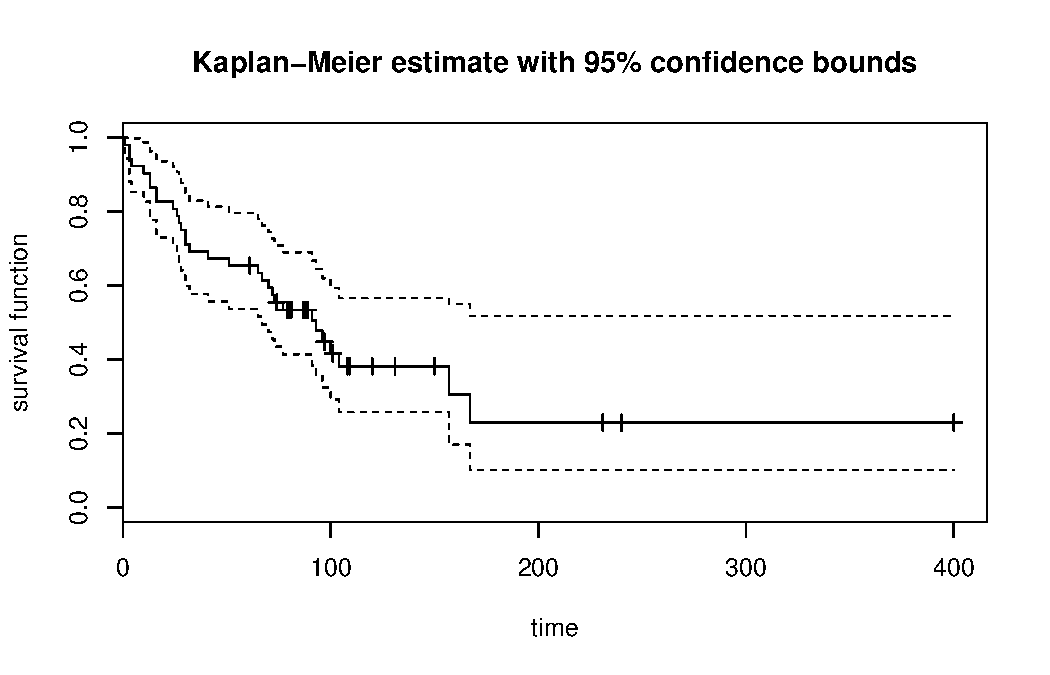
\includegraphics[width=0.66\textwidth]{../figures/kmPlot.pdf} \vspace{-4mm}
\caption{Sample output where only the title, x-axis and y-axis labels have been specified.}
\end{figure}
Sometimes different groups are contained in a single \rcom{Surv} object. For instance, the \rcom{type} variable in the \rcom{tongue} data set describes patient DNA profiles. We can obtain the Kaplan-Meier estimate for each of these groups by regressing the \rcom{Surv} object on the \rcom{type} variable:
{\color{verbatimrcom}\begin{verbatim}
> my.fit1 <- survfit( Surv(time, delta) ~ type )   # here the key is "type"
\end{verbatim}}
(It is also reasonable to use several variables on the right side of the equation.) The summary of \rcom{my.fit1} will contain an additional list item -- \rcom{strata}, accessible via \rcom{summary(my.fit1)\$strata} -- that designates which components of the output correspond to which groups.

Finally, for good coding practices, we detach the \rcom{tongue} data set.
{\color{verbatimrcom}\begin{verbatim}
> detach(tongue)
\end{verbatim}}


\pagebreak

%%% Confidence Bands %%%
\phantomsection
\tTitle{Simultaneous confidence bands} \vspace{-1mm}\par
\tTitle{\rcom{confBands(x, confType="plain", confLevel=0.9, type="ep")}}
\label{confBands}

\emph{Pointwise} confidence intervals, like those introduced in the previous pages, apply to a single point in the time scale. Now we turn our attention to \emph{simultaneous confidence bands} (or \emph{confidence bands} for short), which are valid for the entire range of time values simultaneously. A 95\% confidence band, for example, will capture the entire true survival curve about 19 out of 20 times. 

While the \package{survival} package doesn't offer tools for confidence bands, they may be calculated using \rcom{confBands} from the \package{OIsurv} library. 
% No functions in the \package{survival} package create confidence bands.
%Values describing the confidence bands are obtained using the function \rcom{confBands} from \package{OIsurv}. 
The first argument is a survival object for \rcom{x}, and the other arguments allow customization. The \rcom{confType} may be \rcom{"plain"},  \rcom{"log-log"}, or \rcom{"asin-sqrt"}; the \rcom{confLevel} may be \rcom{0.90}, \rcom{0.95}, or \rcom{0.99}; and the \rcom{type} may be \rcom{"ep"} or \rcom{"hall"} (Hall-Wellner). There are also two optional arguments, \rcom{tL} and \rcom{tU}, that limit the support of the confidence bands. Confidence bands may be added to a plot using the \rcom{lines} function.
{\color{verbatimrcom}\begin{verbatim}
> data(bmt); attach(bmt)
> my.surv <- Surv(t2[group==1], d3[group==1])
> my.cb <- confBands(my.surv, confLevel=0.95, type="hall")
> plot(survfit(my.surv ~ 1), xlim=c(100, 600), xlab="time",
+   ylab="Estimated Survival Function",
+   main="Reproducing Confidence Bands for Example 4.2 in Klein/Moeschberger")
\end{verbatim}}
\begin{figure}[htp]
\centering
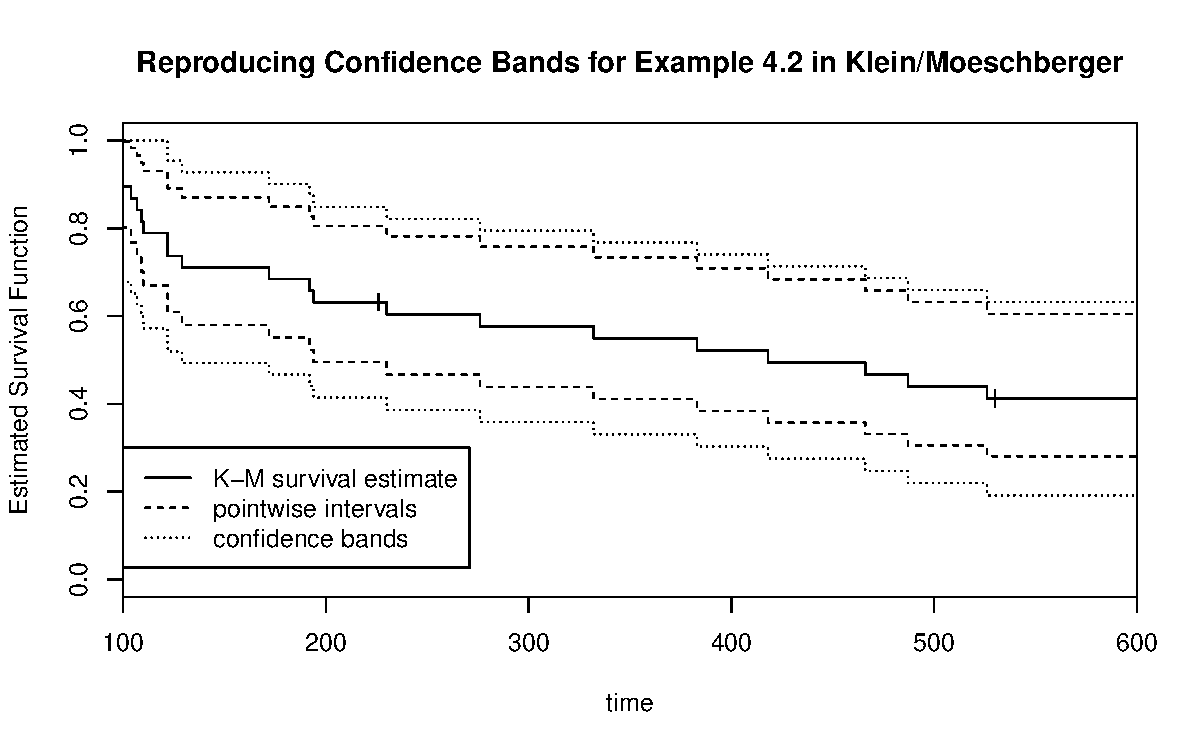
\includegraphics[width=0.81\textwidth]{../figures/confBand.pdf} \vspace{-4mm}
\caption{Confidence intervals and bands. Note that the default for the pointwise confidence bands is a log transformation, which results in asymmetric pointwise confidence intervals.}
\end{figure}
{\color{verbatimrcom}\begin{verbatim}
> lines(my.cb$time, my.cb$lower, lty=3, type="s")
> lines(my.cb$time, my.cb$upper, lty=3, type="s")
> legend(100, 0.3, legend=c("K-M survival estimate",
+   "pointwise intervals","confidence bands"), lty=1:3)
> detach(bmt)
\end{verbatim}}

\pagebreak

%%% Cumulative Hazard %%%
\phantomsection
\tTitle{Cumulative hazard function}
\label{cumulativeHazard}

The cumulative hazard function and the survival function are related in the following way for continuous data:
\begin{align*}
S(t) = \exp\left\{-H(t)\right\}
\end{align*}
The MLE of the hazard function may be obtained by the inverse transformation of the Kaplan-Meier estimate: $\hat{H}(t) = -\log\hat{S}(t)$. Another method to estimate $H(t)$ is the Nelson-Aalen estimator:
\begin{align*}
\tilde{H}(t) &= \sum_{t_i \leq t} \frac{d_i}{Y_i}
		&\sigma_H^2(t) = \sum_{t_i\leq t}\frac{d_i}{Y_i^2}
\end{align*}
While no function in the \package{survival} package calculates either form automatically, the object returned by \rcom{summary(survfit())} can be used to calculate the estimates:
{\color{verbatimrcom}\begin{verbatim}
> data(tongue); attach(tongue)
> my.surv <- Surv(time[type==1], delta[type==1])
> my.fit  <- summary(survfit(my.surv ~ 1))
> H.hat   <- -log(my.fit$surv)
> H.hat   <- c(H.hat, tail(H.hat, 1))
\end{verbatim}}
A summary plot or table may be created using \rcom{H.hat} with \rcom{my.fit\$time}. The Nelson-Aalen estimator may also be constructed:
{\color{verbatimrcom}\begin{verbatim}
> h.sort.of <- my.fit$n.event / my.fit$n.risk
> H.tilde   <- cumsum(h.sort.of)
> H.tilde   <- c(H.tilde, tail(H.tilde, 1))
> plot(c(my.fit$time, 250), H.hat, xlab="time", ylab="cumulative hazard",
+   main="comparing cumulative hazards", ylim=range(c(H.hat, H.tilde)), type="s")
> points(c(my.fit$time, 250), H.tilde, lty=2, type="s")
> legend("topleft", legend=c("H.hat","H.tilde"), lty=1:2)
> detach(tongue)
\end{verbatim}}
\begin{figure}[htp]
\centering
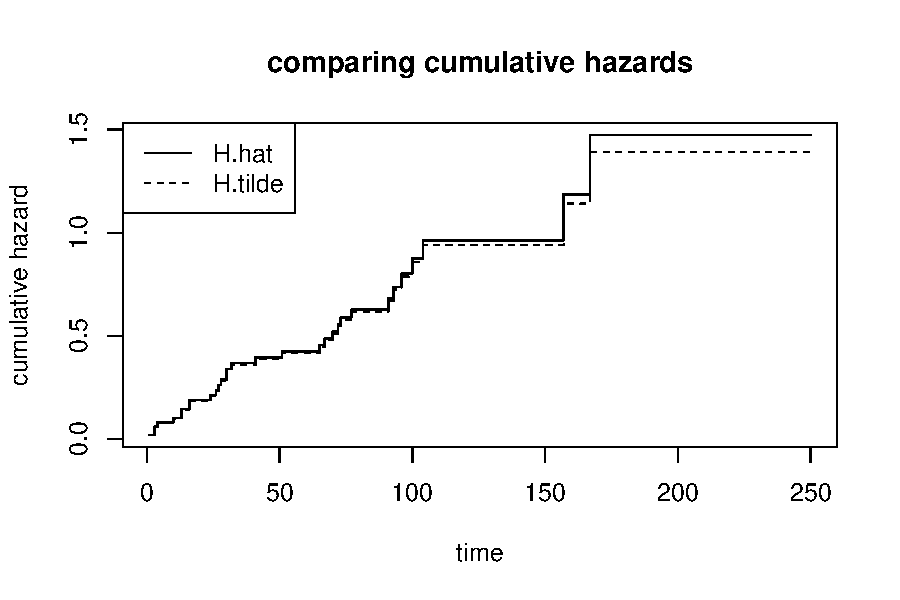
\includegraphics[width=0.57\textwidth]{../figures/cumHazard} \vspace{-4mm}
\caption{Cumulative hazard estimates.}
\end{figure}

\pagebreak

%%% Compute mean and median estimates %%%
\phantomsection
\tTitle{Mean and median estimates with bounds}
\label{meanAndMedianEstimates}

The median survival time is the time $t_{0.5}$ such that $S(t_{0.5}) = 0.5$. This is visualized by graphing the estimated survival function and drawing a horizontal line at 0.5. The estimated median equals the time $\hat{t}_{0.5}$ where the function and line intersect. The confidence interval for $t_{0.5}$ is given by the points at which this horizontal line crosses over the pointwise confidence intervals of $\hat{S}(t)$.

\noindent The mean survival time and its respective estimate are given by
\begin{align*}
\mu &= \int_0^\infty S(t)dt, \qquad\hat{\mu} = \int_0^\infty \hat{S}(t)dt
\end{align*}
If $S(t)$ (or $\hat{S}(t)$) does not converge to zero, the integral diverges. This property creates a challenge for most data, and one resolution is to use a finite value $\tau$ as the bound for the integral, where $\tau$ may represent the maximum survival time considered to be possible. Another reasonable choice for $\tau$ is the maximum observed or censored time. Using a finite $\tau$ results in a new statistic and corresponding estimate: $\mu_\tau = \int_0^\tau S(t)dt$. Letting $t_i$, $Y_i$, $d_i$, and $D$ be as described in the \hyperref[kapMeiEstimateAndBounds]{Kaplan-Meier section}, the estimated variance of $\hat{\mu}_\tau$ is
\begin{eqnarray*}
\widehat{V}(\hat{\mu}_\tau) = \sum_{i=1}^D\left[\int_{t_i}^\tau \hat{S}(t)dt\right]^2 \frac{d_i}{Y_i(Y_i-d_i)}
\end{eqnarray*}

The median and its 95\% confidence interval may be estimated using \rcom{survfit()}:
{\color{verbatimrcom}\begin{verbatim}
> data(drug6mp); attach(drug6mp)
> my.surv <- Surv(t1, rep(1, 21))   # all placebo patients observed
> survfit(my.surv ~ 1)
Call: survfit(formula = my.surv ~ 1)

records   n.max n.start  events  median 0.95LCL 0.95UCL 
     21      21      21      21       8       4      12 
\end{verbatim}}
Using \rcom{survfit()} in conjunction with \rcom{print()}, the mean survival time and its standard error may be obtained:
{\color{verbatimrcom}\begin{verbatim}
> print(survfit(my.surv ~ 1), print.rmean=TRUE)
Call: survfit(formula = my.surv ~ 1)

   records      n.max    n.start     events     *rmean  *se(rmean)    median 
     21.00      21.00      21.00      21.00       8.67       1.38       8.00 
   0.95LCL    0.95UCL 
      4.00      12.00 
    * restricted mean with upper limit =  23 
> detach(drug6mp)
\end{verbatim}}
The \rcom{print.rmean=TRUE} argument is used to obtain the mean and its standard error, and $\tau$ is automatically set as the largest observed or censored time. Alternatively, $\tau$ may be specified using the \rcom{rmean} argument.

\pagebreak

%%% Test difference of 2 survival curves %%%
\phantomsection
\tTitle{Tests for two or more samples} \vspace{-1mm}\par
\tTitle{\rcom{survdiff(formula, rho=0)}}
\label{testsForTwoOrMoreSamples}

Given two or more samples, is there a statistical difference between the survival times? We can formulate the hypotheses in the context of hazard functions as
\begin{itemize}
\item $H_0: h_1(t) = h_2(t) = \cdots = h_n(t)$ for all $t$, and
\item $H_A: h_i(t_0)\neq h_j(t_0)$ for at least one pair $i,j$ and time $t_0$.
\end{itemize}
Let
\begin{itemize}
\item $t_{i}$ be times where events are observed (assume these are ordered and there are $D$ such times),
\item $d_{ik}$ be the number of observed events from group $k$ at time $t_i$,
\item $Y_{ik}$ be the number of subjects in group $k$ that are at risk at time $t_i$ (see \hyperref[kapMeiEstimateAndBounds]{K-M section}),
\item $d_{i} = \sum_{j=1}^n d_{ij}$,
\item $Y_{i} = \sum_{j=1}^n Y_{ij}$, and
\item $W(t_i)$ be the weight of the observations at time $t_i$.
\end{itemize}
Then to test the hypothesis above, a vector $Z$ is computed, where the $k^{th}$ element is
\begin{eqnarray*}
Z_k = \sum_{i=1}^D W(t_i)\left[d_{ik} - Y_{ik}\frac{d_{i}}{Y_{i}}\right]
\end{eqnarray*}
The covariance matrix $\widehat{\Sigma}$ is also computed from the data (see reference~\ref{Klein2003}). Under the null hypothesis, the test statistic $X^2 = Z'\hat{\Sigma}^{-1}Z$ follows a $\chi^2$ distribution with $n$ degrees of freedom. That is, if $X^2 > \chi^2_{1-\alpha, df=n}$, the data provide strong evidence against the null hypothesis and we reject~$H_0$.

The function \rcom{survdiff()} is used for this hypothesis test. The first argument is a survival object against a categorical covariate variable that is typically a variable designating which groups correspond to which survival times. The object returned by \rcom{survdiff()} provides useful information. (Surprisingly, the summary of this object is not particularly useful.)
{\color{verbatimrcom}\begin{verbatim}
> data(btrial); attach(btrial)       # time variable warning omitted
> survdiff(Surv(time, death) ~ im)   # output omitted
\end{verbatim}}
The second \rcom{survdiff()} argument, \rcom{rho}, designates the weights according to $\hat{S}(t)^\rho$ and may be any numeric value. The default is \rcom{rho=0} and corresponds to the log-rank test. The \term{Peto \& Peto modification of the Gehan-Wilcoxon test} is computed using \rcom{rho=1}:
{\color{verbatimrcom}\begin{verbatim}
> survdiff(Surv(time, death) ~ im, rho=1)   # some output omitted
...

 Chisq= 4.4  on 1 degrees of freedom, p= 0.037 
> detach(btrial)
\end{verbatim}}
To give greater weight to the first part of the survival curves, use \rcom{rho} larger than \rcom{0}. To give weight to the later part of the survival curves, use \rcom{rho} smaller than \rcom{0}. The output of \rcom{survdiff()} is generally self-explanatory. A $\chi^2$ statistic is computed along with a p-value.

\pagebreak

%%% Cox PH Models %%%
\phantomsection
\tTitle{Cox proportional hazards model, constant covariates} \vspace{-1mm} \par
\tTitle{\rcom{coxph(formula, method)}}
\label{coxPHConstCov}

The Cox proportional hazards (Cox PH) model fits survival data with covariates $z$ to a hazard function of the form
\begin{eqnarray*}
h(t|z) = h_0(t)\exp\left\{ \beta'z  \right\}
\end{eqnarray*}
where $\beta$ is an unknown vector and $h_0(t)$ is the \textit{baseline hazard}, which is nonparametric. Primary interest lies in estimating the parameter $\beta$ using the partial likelihood:
\begin{eqnarray*}
L(\beta) = \prod_{i=1}^D \frac{\exp\left[\beta'z_{(i)}\right]}{\sum_{j \in R(t_i)}\exp\left\{\beta'z_j\right\}}
		\quad
		\text{where }R(t_i)\text{ is the ``risk set'' at time }t_i.
\end{eqnarray*}
The MLE $\hat{\beta}$ (a vector) is asymptotically $N(\beta, I^{-1})$, where $I$ represents the Fisher information. This normal approximation makes doing local tests possible. A \term{local test} examines a subset of the elements of $\beta$, testing the claim $C\beta = d$, where $C$ is a $q\times p$ matrix of full rank and $d$ is a vector of length $q$. For example, we could set up a very simple test for $\beta_1=0$ by choosing $C_{1 \times p}=(1,0,0,...,0)$ and $d_{1 \times 1}=0$. For a general $C$ and $d$, the test statistic~is
\begin{eqnarray*}
X_W^2 = \left(C\hat{\beta} - d\right)'\left[C\hat{I}^{-1}C'\right]^{-1}\left(C\hat{\beta} - d\right),
\end{eqnarray*}
which under the null hypothesis follows $\chi^2_q$. This is known as the \term{Wald test}.

Beyond obtaining test p-values, there may be interest in the survival function for particular covariates. If the estimate of the baseline survival function $\hat{S}_0(t)$ is provided, then the estimate of the survival function for an individual with covariates $z_k$ may be obtained via
\begin{eqnarray*}
\hat{S}(t|z_k) = \left[\hat{S}_0(t)\right]^{\exp\left(\hat{\beta}'z_k \right)}
\end{eqnarray*} 

The function \rcom{coxph()} fits a Cox PH model to the supplied data. The first argument is a formula, where the response is a survival object. %The second argument, \rcom{method}.
{\color{verbatimrcom}\begin{verbatim}
> data(burn); attach(burn)
> my.surv   <- Surv(T1, D1)
> coxph.fit <- coxph(my.surv ~ Z1 + as.factor(Z11), method="breslow")
> coxph.fit
Call:
coxph(formula = my.surv ~ Z1 + as.factor(Z11), method = "breslow")


                  coef exp(coef) se(coef)     z     p
Z1               0.497     1.644    0.208  2.38 0.017
as.factor(Z11)2 -0.877     0.416    0.498 -1.76 0.078
as.factor(Z11)3 -1.650     0.192    0.802 -2.06 0.040
as.factor(Z11)4 -0.407     0.666    0.395 -1.03 0.300

Likelihood ratio test=14.6  on 4 df, p=0.00569  n= 154, number of events= 99 
\end{verbatim}}
Two covariates have been used in this example. The second argument listed, \rcom{method}, specifies how ties are handled. The default is \rcom{"efron"}, and the other options are \rcom{"breslow"} and \rcom{"exact"}. Much useful information is obtained in the summary of \rcom{coxph()}, including
\begin{itemize}
\item estimates of the $\beta_k$, including standard errors and p-values for each test $H_0: \beta_k=0$, % with the other $\beta_j = \hat{\beta}_j$,
\item an estimate of the risk ratio and its confidence interval, and
\item p-values for likelihood ratio, Wald, and score tests for the global null, $H_0: \beta_i =0$ for all $i$.
\end{itemize}
More complex hypotheses may be checked using other items from the model fit:
{\color{verbatimrcom}\begin{verbatim}
> co <- coxph.fit$coefficients  # may use coxph.fit$coeff instead
> va <- coxph.fit$var           # I^(-1), estimated cov matrix of the estimates
> ll <- coxph.fit$loglik        # log-likelihood for alt and null MLEs, resp.
\end{verbatim}}
To obtain the baseline survival function from a Cox PH model, apply \rcom{survfit()} to \rcom{coxph()}:{\color{verbatimrcom}\begin{verbatim}
> my.survfit.object <- survfit(coxph.fit)
\end{verbatim}}
The object returned by \rcom{survfit()} has the familiar characteristics and properties as before. For instance, the baseline survival function may be plotted using the \rcom{plot()} function.

Here we will run one local test. Above, \rcom{Z11} was a factor variable represented as the second, third, and fourth coefficients of \rcom{coxph.fit}. We first construct $C$ and $d$, then we compute the test statistic~$X^2_W$. In the code below, the objects \rcom{t1} and \rcom{t2} were computed as intermediate steps for obtaining the test statistic.
{\color{verbatimrcom}\begin{verbatim}
> C   <- matrix(c(0, 1, 0, 0,
+                 0, 0, 1, 0,
+                 0, 0, 0, 1), nrow=3, byrow=TRUE)
> d   <- rep(0, 3)
> t1  <- C %*% co - d
> t2  <- C %*% va %*% t(C)
> XW2 <- c(t(t1) %*% solve(t2) %*% t1)
> pchisq(XW2, 3, lower.tail=FALSE)
[1] 0.1025018
> detach(burn)
\end{verbatim}}
The concatenation function \rcom{c()} used in the computation of \rcom{XW2} makes \rcom{XW2} a vector rather than a $1\times1$ matrix. The p-value of the test is 0.103, meaning \rcom{Z11} is not statistically significant for a significance level of $\alpha=0.05$.

For a more thorough discussion of Cox PH models in~\R{}, please see reference~\ref{Fox2002}.

\pagebreak

%%% Cox PH time-dependent Models %%%
\phantomsection
\tTitle{Cox proportional hazards model, time-dependent covariates}
\label{coxPHTimeDepCov}

Using time-dependent covariates in \R{} is an exercise in organization. Previously considered covariates were unchanging attributes, such as treatment group or control group or a patient's race. Now we consider time-dependent covariates, such as interventions or environmental factors that might result in a change mid-study.

To use time-dependent covariates in \R{}, we apply left-truncation liberally. For example, if there is an intervention for patient $i$, then we split patient $i$ into two separate observations: pre and post-intervention. More explicitly, suppose the patient intervention took place at time $t_{i} = 45$ and the event for patient $i$ was observed at $t_{event}=58$. We would split this patient's record into two pieces: 0 to 45 and 45 to 58. The covariate for intervention can be assigned different values for each interval. Applying this time-splitting method in~\R{} requires care. Start and end times for each interval are constructed, and right-censoring must be tracked for each pair of start/end times.

We consider the following example (simulated data). Patient records from an alcohol abuse clinic were obtained for 150 days after the patients became sober. The event of interest was alcohol-relapse, and four variables were available. The \rcom{event} variable describes the observed or censored relapse time; the \rcom{delta} variable describes whether the event was observed (\rcom{TRUE}) or censored (\rcom{FALSE}); \rcom{gender} is a time-independent covariate; and \rcom{int} is a time-dependent covariate indicating whether the patient had an intervention, where some patients relapsed before their scheduled interventions and so have \rcom{NA} listed. All interventions occurred \emph{after} the patients became sober (day 0). That is, the intervention covariate changed for each patient over time, so long as they didn't relapse first. These data are saved as \rcom{relapse} in the \rcom{OIsurv} package.
{\color{verbatimrcom}\begin{verbatim}
> data(relapse)
> relapse
    time event gender int
1    150 FALSE      0  84
2     53  TRUE      1  50
3     12  TRUE      1  NA
4    150 FALSE      0  89
5    150 FALSE      1  77
...
299   10  TRUE      0  NA
300   94  TRUE      1   4
\end{verbatim}}

These data can be modeled using two steps:
\begin{enumerate}
\item Construct survival records that may include left and right-censored observations. The survival record of each patient with an intervention is broken into two survival records: one before the intervention and one after. This step is largely book-keeping and programming in \R{}.
\item The new survival records can be run through the \rcom{coxph()} function.
\end{enumerate}
We first initialize new vectors to represent variables of the survival records. The variables \rcom{t1} and \rcom{t2} represent start and end times, respectively, \rcom{d} represents whether relapse was observed (\rcom{TRUE}) or right-censored (\rcom{FALSE}), \rcom{g} represents gender, and \rcom{i} represents whether the patient was undergoing the intervention treatment (we must be mindful not to overwrite this variable in a loop).
{\color{verbatimrcom}\begin{verbatim}
> N  <- dim(relapse)[1]
> t1 <- rep(0, N+sum(!is.na(relapse$int)))  # initialize start time at 0
> t2 <- rep(-1, length(t1))                 # build vector for end times
> d  <- rep(-1, length(t1))                 # whether event was censored
> g  <- rep(-1, length(t1))                 # gender covariate
> i  <- rep(FALSE, length(t1))              # initialize intervention at FALSE
\end{verbatim}}
Next, each patient is checked for whether they had an intervention. If they did not, then their record is simply copied to the new variables used. If there was an intervention, their observations are split into two pieces: the period prior to intervention and the period after intervention. The period after intervention is left-truncated for the time of intervention.
{\color{verbatimrcom}\begin{verbatim}
> j  <- 1
> for(ii in 1:dim(relapse)[1]){
+   if(is.na(relapse$int[ii])){      # no intervention, copy survival record
+     t2[j] <- relapse$event[ii]
+     d[j]  <- relapse$delta[ii]
+     g[j]  <- relapse$gender[ii]
+     j <- j+1
+   } else {                         # intervention, split records
+     g[j+0:1] <- relapse$gender[ii] # gender is same for each time
+     d[j]     <- 0                  # no relapse observed pre-intervention
+     d[j+1]   <- relapse$delta[ii]  # relapse occur post-intervention?
+     i[j+1]   <- TRUE               # intervention covariate, post-intervention
+     t2[j]    <- relapse$int[ii]-1  # end of pre-intervention
+     t1[j+1]  <- relapse$int[ii]-1  # start of post-intervention
+     t2[j+1]  <- relapse$event[ii]  # end of post-intervention
+     j <- j+2                       # two records added
+   }
+ }
\end{verbatim}}
The meanings of the variables are as follows: \rcom{t1} represents the start of each interval; \rcom{t2} the end of each interval; \rcom{e} indicates if the event was observed; \rcom{g} is the gender covariate; and \rcom{i} is the indicator variable for whether this interval is associated with a patient post-intervention.

While many patients had time-varying covariates (namely, the intervention), each of the new intervals has covariates that do not change, which allows for the survival object and Cox PH model to be constructed:
{\color{verbatimrcom}\begin{verbatim}
> mySurv <- Surv(t1, t2, d)        # pg 3 discusses left-trunc. right-cens. data
> myCPH  <- coxph(mySurv ~ g + i)
\end{verbatim}}

This example was a simple case; there was a single time-dependent covariate, and it changed at most once per case. In some instances, there may be many time-varying covariates, even some that change every time unit. In most of these instances, the same method may be used. Whenever a covariate changes from one time unit to the next, split the interval into two and use left-truncation and right-censoring as needed.

For additional reading on time-dependent covariates in \R{}, see pages 7-11 of reference~\ref{Fox2002}.

%One case of interest is creating a new time-dependent covariate, $Z_i^t$, from another covariate, $Z_i$. This may be done by using a transformation on the time and multiply the result by $Z_i$:
%\begin{eqnarray*}
%Z_i^t = Z_i * transformation(t)
%\end{eqnarray*}
%A common transformation is $\log$ but others may be used. A function to create a type of variable of this form and also to run a Cox PH model with it is the following:
%{\color{verbatimrcom}\begin{verbatim}
%timeDepCoxph(x, colTime, colDelta, colCov, tdCov, transform=log,
%   outputModel=TRUE, outputDF=FALSE, verbose=TRUE, ...)
%\end{verbatim}}
%The function is included in the \package{OIsurv} package. Here,
%\begin{itemize}
%\item \rcom{x} is a data frame with all of the original data,
%\item \rcom{colTime} is the name/number indicating which column of \rcom{x} is the event/right-censored time,
%\item \rcom{colDelta} is the name/number representing the column of \rcom{x} indicates observed events,
%\item \rcom{colCov} is a vector of the column numbers/names of the covariates to be included in the model, and
%\item \rcom{tdCov} is the column number/name of the covariate $Z_i$ to be used to create the time-dependent covariate. $Z_i$ must be a vector with only 2 unique numerical values. (e.g. $Z_i$ is a vector of \rcom{0}'s and \rcom{1}'s).
%\end{itemize}
%The following arguments have defaults, as are specified above:
%\begin{itemize}
%\item \rcom{transform} is the type of transformation to be used on time,
%\item \rcom{outputModel} indicates whether the Cox PH model should be included in the output,
%\item \rcom{outputDF} indicates whether the time-dependent data frame that was created should be output (this may be useful if many closely related models are going to be checked), and
%\item \rcom{verbose} indicates whether the user should be notified at how far along the function is at computing the data frame to be used in the Cox PH model (this is useful to see how fast the function is running).
%\item Additional arguments are passed to \rcom{coxph()},
%\end{itemize}
%Below is an example of how to use this function:
%{\color{verbatimrcom}\begin{verbatim}
%> data(burn)
%> attach(burn)
%> td.coxph <- timeDepCoxph(burn, 'T1', 'D1', 2:4, 'Z1', verbose=FALSE)
%\end{verbatim}}
%The covariates in the output will be of the same order as specified in \rcom{colCov}.
%{\color{verbatimrcom}\begin{verbatim}
%> td.coxph   # some model output is omitted for brevity
%...
%                coef exp(coef) se(coef)      z      p
%Z1            1.3569     3.884    0.719  1.886 0.0590
%Z2            0.6899     1.994    0.231  2.981 0.0029
%Z3            0.0496     1.051    0.302  0.164 0.8700
%time.dep.cov -0.3383     0.713    0.312 -1.085 0.2800
%\end{verbatim}}
%The default output of \rcom{timeDepCoxph()} is the output of \rcom{coxph()}. It has all the usual outputs of \rcom{coxph()}. For example, log-likelihood:
%{\color{verbatimrcom}\begin{verbatim}
%> td.coxph$loglik
%[1] -420.4825 -411.8814
%> detach(burn)
%\end{verbatim}}

\pagebreak




% - - - - - AFT models  - - - - - %
\phantomsection
\tTitle{Accelerated failure-time models} \vspace{-1mm} \par
\tTitle{\rcom{survreg(formula, dist='weibull')}}
\label{accFailureTimeModels}

An accelerated failure-time (AFT) model is a parametric model with covariates and failure times following the survival function of the form $S(x|Z) = S_0\left(x*\exp\left[ \theta'Z \right]\right)$, where $S_0$ is a function for the baseline survival rate. The term $\exp\left[\theta'Z\right]$ is called the \term{acceleration factor}. The AFT model uses covariates to place individuals on different time scales -- note the scaling by the covariates in $S(t|Z)$ via $\exp\left[ \theta'Z \right]$. The AFT model can be rewritten in a log-linear form, where the log of failure time (call this $\log X$) is linearly related to the mean $\mu$, the acceleration factor, and an error term~$\sigma W$:
\begin{eqnarray*}
\log X = \mu - \theta'Z + \sigma W
\end{eqnarray*}
%The main choice to be made is which distribution to use for the error. The options discussed in Klein and Moeschberger are shown in the table below:
$W$ describes the error distribution. The following models for $W$ are discussed in reference~\ref{Klein2003}:
\begin{quotation}\center
\begin{tabular}{llccc}
\hline 
\hline
Distribution & \rcom{  } & df &\ & Included in \package{survival}? \\
\hline 
exponential & & 1 && yes \\
Weibull & & 2 && yes \\
lognormal & & 2 && yes \\
log logistic & & 2 && yes \\
generalized gamma & & 3 && no \\
\hline
\hline
\end{tabular}
\end{quotation}

The \rcom{survreg()} function from the \package{survival} package is used for AFT modeling. The first argument is \rcom{formula}, where a survival object is regressed on predictors. The argument \rcom{dist} has several options to describe the parametric model used (\rcom{"weibull"}, \rcom{"exponential"}, \rcom{"gaussian"}, \rcom{"logistic"}, \rcom{"lognormal"}, or \rcom{"loglogistic"}). The code below follows Example 12.2 from reference~\ref{Klein2003} and uses a~Weibull model:
{\color{verbatimrcom}\begin{verbatim}
> data(larynx)
> attach(larynx)
> srFit <- survreg(Surv(time, delta) ~ as.factor(stage) + age, dist="weibull")
> summary(srFit)
...
                    Value Std. Error      z        p
(Intercept)        3.5288     0.9041  3.903 9.50e-05
as.factor(stage)2 -0.1477     0.4076 -0.362 7.17e-01
as.factor(stage)3 -0.5866     0.3199 -1.833 6.68e-02
as.factor(stage)4 -1.5441     0.3633 -4.251 2.13e-05
age               -0.0175     0.0128 -1.367 1.72e-01
Log(scale)        -0.1223     0.1225 -0.999 3.18e-01

Scale= 0.885 

Weibull distribution
Loglik(model)= -141.4   Loglik(intercept only)= -151.1
	Chisq= 19.37 on 4 degrees of freedom, p= 0.00066 
Number of Newton-Raphson Iterations: 5 
n= 90 
\end{verbatim}}
In the output, \rcom{(Intercept)} and \rcom{Log(scale)} correspond to estimates of $\mu$ and $\log\sigma$. The other estimates correspond to covariate coefficients. We might also consider an exponential model:
{\color{verbatimrcom}\begin{verbatim}
> srFitExp <- survreg(Surv(time, delta) ~ as.factor(stage) + age, dist="exponential")
> summary(srFitExp)
...
                    Value Std. Error      z        p
(Intercept)        3.7550     0.9902  3.792 1.49e-04
as.factor(stage)2 -0.1456     0.4602 -0.316 7.52e-01
as.factor(stage)3 -0.6483     0.3552 -1.825 6.80e-02
as.factor(stage)4 -1.6350     0.3985 -4.103 4.08e-05
age               -0.0197     0.0142 -1.388 1.65e-01

Scale fixed at 1 

Exponential distribution
Loglik(model)= -141.9   Loglik(intercept only)= -151.1
	Chisq= 18.44 on 4 degrees of freedom, p= 0.001 
Number of Newton-Raphson Iterations: 4 
n= 90 
\end{verbatim}}
%The AIC for the exponential is 293.8 ($p=5$). Because the $293.8 < 294.8$, the AIC suggests the exponential model may be more appropriate.

When $\sigma=1$, the Weibull model is equivalent to the exponential model. We consider two strategies for choosing the final model:
\begin{itemize}
\item a likelihood ratio test, which evaluates the null hypothesis $\sigma=1$ against the two-sided alternative, and
\item examination of the significance of the \rcom{Log(scale)} coefficient (see the output to \rcom{summary(srFit)}).
\end{itemize}
In the example, both approaches result in the same conclusion: there is insufficient evidence to reject the hypothesis that $\sigma=1$ ($H_0$). For this reason, we would likely go with the simpler exponential~model.

Interested users may explore the many stored components in a \rcom{survreg()} object:
{\color{verbatimrcom}\begin{verbatim}
> # the output is omitted from each command below
> srFitExp$coeff    # covariate coefficients
> srFitExp$icoef    # intercept and scale coefficients
> srFitExp$var      # variance-covariance matrix
> srFitExp$loglik   # log-likelihood
> srFit$scale       # not using srFitExp (defaulted to 1)
\end{verbatim}}
Finally, we should not forget to detach the data set.
{\color{verbatimrcom}\begin{verbatim}
> detach(larynx)
\end{verbatim}}

\pagebreak

%\tTitle{Acknowledgements}

%\vspace{4mm}

%Thank you to Gang Li, who taught me everything I know about survival analysis and encouraged me to write this guide for my course project.

%\vspace{15mm}

\phantomsection

\tTitle{Acknowledgements}

\vspace{4mm}

Thank you to Beau Benjamin Bruce, who has kindly provided a function useful for Cox PH models with time-dependent covariates to be hosted at OpenIntro (\href{http://www.openintro.org/stat/surv.php}{www.openintro.org/stat/surv.php}). This new function greatly improves on a function used in the first version of this guide.

Thank you also to Christopher Barr for his helpful comments on the revisions for this guide.

\vspace{15mm}

\tTitle{References}
\label{references}

\vspace{4mm}

\bibItem{survivalPackage}{Terry Therneau and original Splus$->$\R{} port by Thomas Lumley (2011). survival: Survival analysis, including penalised likelihood. \R{} package version 2.36-10. \vspace{-2mm}\par \url{http://CRAN.R-project.org/package=survival}.}

\bibItem{R}{\R{} Development Core Team (2010). \R{}: A language and environment for statistical computing. \R{} Foundation for Statistical Computing, Vienna, Austria. ISBN 3-900051-07-0, URL \url{http://www.R-project.org.}}

\bibItem{OIsurv}{David M Diez (2012).
  OIsurv: Supplement to survival analysis tutorial. \R{} package
  version 1.0. \url{http://CRAN.R-project.org/package=OIsurv}}

\bibItem{KMsurvPackage}{Original by Klein, Moeschberger and modifications by Jun Yan (2010). KMsurv: Data sets from Klein and Moeschberger (1997), Survival Analysis. \R{} package version 0.1-4. \vspace{-2mm}\par \url{http://CRAN.R-project.org/package=KMsurv}.}

\bibItem{Klein2003}{Klein, John P., and Melvin L. Moeschberger. Survival Analysis: Techniques for Censored and Truncated Data. New York: Springer, 2003.}

\bibItem{formsOfSurvData}{ReliaSoft Corporation website (2006). Data Classification. \vspace{-2mm}\par \url{http://www.weibull.com/LifeDataWeb/data_classification.htm}}.

\bibItem{Fox2002}{Fox, John 2002. Cox Proportional-Hazards Regression for Survival Data. Appendix to An \R{} and S-PLUS Companion to Applied Regression.}

\vspace{15mm}

\tTitle{Additional resources}

\vspace{4mm}

\bibItem{Lumley2007}{Lumley, Thomas, 2007. The Survival Package (\R{} help guide).}







\end{document}   